\documentclass[a4paper]{article}

\usepackage{graphicx}

\usepackage{FillAFour}
\usepackage{HaskellVerb}
\usepackage{hyperref}
\usepackage{listings}



\begin{document}

\title{JSON Parser and Validator}

\author{Caleb Howard}

\maketitle

\begin{abstract}
   \noindent This document covers the JSON Parser and Validator haskell program. It highlights the
   use cases of the program and explains key sections in the source code. EBNF diagrams are included 
   to illustrate the parser syntax.
\end{abstract}

\section{Introduction}

The JSON Parser and Validator haskell program is responsible for parsing and comparing two JSON documents.
The program reads a JSON data document and a JSON schema document.
After parsing both documents into separate parse trees, both parses trees are used to 
verify that the schema document is a valid schema for the data document. \newline
Before constructing the parser, EBNF diagrams were created to illustrate the lexical and context-free
syntax of a JSON document. The Syntrax tool was used to generate the syntax (railroad) diagrams from
.ebnf productions. For more information or to view these diagrams, refer to section \hyperref[sec:syntax]{2, Syntax}.


% SYNTAX SECTION ----------------------------------
\section{Syntax}
\label{sec:syntax}

EBNF and syntax diagrams for JSON Documents:

% Lexical Subsection ----------------------------------
\subsection{Lexical Syntax}

\subsubsection{JsonL - All JSON document lexemes}

\EBNFInput{syntax/Lexical/jsonL.ebnf}

{\centering

   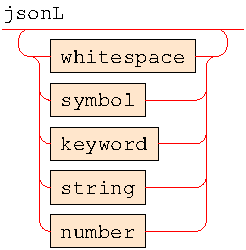
\includegraphics[scale=0.9]{syntax/Lexical/jsonL}

}
\newpage

\subsubsection{Symbol}

\EBNFInput{syntax/Lexical/symbol.ebnf}

{\centering

   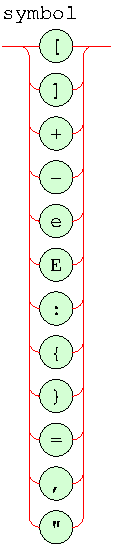
\includegraphics[scale=0.9]{syntax/Lexical/symbol}

}

\subsubsection{String}

\EBNFInput{syntax/Lexical/string.ebnf}

{\centering

   
\includegraphics[scale=0.9]{syntax/Lexical/string}

}

\subsubsection{Keyword}

\EBNFInput{syntax/Lexical/keyword.ebnf}

{\centering

   
\includegraphics[scale=0.9]{syntax/Lexical/keyword}

}

\newpage

\subsubsection{Number}

\EBNFInput{syntax/Lexical/number.ebnf}

{\centering

   
\includegraphics[scale=0.9]{syntax/Lexical/number}

}

\subsubsection{Whitespace}

\EBNFInput{syntax/Lexical/whitespace.ebnf}

{\centering

   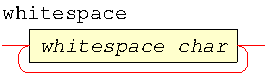
\includegraphics[scale=0.9]{syntax/Lexical/whitespace}

}
\newpage

% Context-Free Subsection ----------------------------------
\subsection{Context-Free Syntax}

\subsubsection{Json}

\EBNFInput{syntax/ContextFree/json.ebnf}

{\centering

   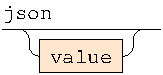
\includegraphics[scale=0.9]{syntax/ContextFree/json}

}

\subsubsection{Array}

\EBNFInput{syntax/ContextFree/array.ebnf}

{\centering

   
\includegraphics[scale=0.9]{syntax/ContextFree/array}

}

\subsubsection{Member}

\EBNFInput{syntax/ContextFree/member.ebnf}

{\centering

   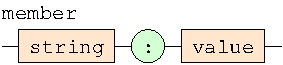
\includegraphics[scale=0.9]{syntax/ContextFree/member}

}

\subsubsection{Object}

\EBNFInput{syntax/ContextFree/object.ebnf}

{\centering

   
\includegraphics[scale=0.9]{syntax/ContextFree/object}

}

\subsubsection{Value}

\EBNFInput{syntax/ContextFree/value.ebnf}

{\centering

   
\includegraphics[scale=0.9]{syntax/ContextFree/value}

}

\newpage

% CODE SECTION ----------------------------------------
\section{Code}

\subsection{JsonTypes Module}

The JsonTypes module holds Haskell data types for JSON data. These types are
used by the the JsonParser and JsonValidator modules. The JsonMember type
holds information for a JSON object's member, it consists of a String and JsonValue.
The JsonValue data type is a recursive type, it holds data for items that 
can either be standalone in a JSON document, or can be a value in a "string":value
JSON member.

\VerbatimInput{src/JsonTypes.hs}
\newpage

\subsection{JsonParser Module}

The JsonParser module handles all parsing of a given JSON document. It uses the ABR library
to construct lexers and parsers which correlate to the syntax diagrams listed in section
\hyperref[sec:syntax]{2, Syntax}. The parsers use the produced lexemes to create parse trees for two documents, or
if any JSON syntax errors exist, a relevant error message will be displayed.
The filenames of the two JSON documents are passed as command line arguments. The first command line argument is a reference to 
a JSON data document, the second is a reference to a JSON schema document, which is to
be used by the JsonValidator module to validate the schema against the data document.
Ultimately, this module will print whether the schema validation was successful or failed.


\VerbatimInput{src/JsonParser.hs}
\newpage

\subsection{JsonValidator Module}

The JsonValidator module handles the verification of a provided JSON schema document against
a provided JSON data document. The module uses the parse trees created in
the JsonParser. Firstly, the parse tree of the JSON schema is compiled into a different tree structure. 
The compilation involves converting all the \{string : value\} objects into JsonSchema types.
The compilation stage also loads any custom schema types using the JsonSchemaObject data constructor.
To further understand how to the JsonSchemaObject data constructor works, refer to the code comments surrounding 
its definition.\newline
The compilation is done to make the pattern matching in the validate function more readable and neat.
\newline\newline
For the most part, the validate function uses only pattern matching. However, when we encounter a
JsonSchemaObject JsonObject pattern match, we must also confirm the JsonObject has a 1 to 1 matching
for its members and the customTypes defined in the schema. Refer to the code comments in the code piece 
below for a step by step explanation of how this part of validation was implemented.


\VerbatimInput{src/JsonValidator.hs}



\end{document}
